\documentclass[conference]{IEEEtran}
\IEEEoverridecommandlockouts
\renewcommand\IEEEkeywordsname{Palabras clave}
\usepackage{amsmath,amssymb,amsfonts}
\usepackage{algorithmic}
\usepackage{graphicx}
\usepackage{caption}
\usepackage{subcaption}
\usepackage{textcomp}
\usepackage{xcolor}
\usepackage{url}
\usepackage{multirow}
\usepackage{booktabs}
\usepackage{hyperref}
\usepackage{makecell}

\hypersetup{
    colorlinks=true,
    linkcolor=black,
    filecolor=black,      
    citecolor=black,
    urlcolor=blue,
    pdftitle={Abbate (2026). Ordinal Aerial Imagery for Longitudinal Neighborhood Wealth Tracking},
    }
\usepackage{booktabs}
\usepackage{natbib}

\newcommand{\linebreakand}{%
  \end{@IEEEauthorhalign}
  \hfill\mbox{}\par
  \mbox{}\hfill\begin{@IEEEauthorhalign}
}

\def\BibTeX{{\rm B\kern-.05em{\sc i\kern-.025em b}\kern-.08em
    T\kern-.1667em\lower.7ex\hbox{E}\kern-.125emX}}


\newcommand{\source}[1]{\caption*{{#1}} }

\begin{document}
% \urlstyle{same}

% \title{\huge \textbf{Una estimación geográfica del ingreso per cápita del AMBA utilizando imágenes satelitales}* \\
\title{\huge \textbf{Ordinal Aerial Imagery for Longitudinal Neighborhood Wealth Tracking}: A Building-Level Ranking Approach Applied to New York City
} 

\author{\IEEEauthorblockN{Nicolás F. Abbate}
\IEEEauthorblockA{\textit{New York University} \\
abbate.nicolas@nyu.edu}
% \textbf{TODO: add co-authors if applicable}
}

% \onecolumn % switch to one-column layout
\maketitle

\begin{abstract}
Tracking neighborhood-level wealth over time is difficult even in survey-rich settings: small-area income estimates are noisy and are contaminated by aggregate macroeconomic shifts that obscure genuine local change. We develop a method that recovers the relative wealth of individual buildings from high-resolution aerial imagery alone. Rather than predicting income in levels—which conflates local capital accumulation with city-wide trends—we train a model to rank buildings within each city and year, supervising only the direction of pairwise comparisons and never their magnitude. This ordinal design is invariant to aggregate drift and transfers across cities with different income distributions without retraining. Applied to New York City over 2010–2024, the model attains a Spearman correlation of 0.85 with census-tract income in a spatial area and calendar year withheld from training. A staggered difference-in-differences event study shows that predicted scores respond to new construction in a dose-dependent manner, evidence that the model captures structural change rather than pre-existing trends. Mapping the ordinal scores onto local survey quantiles delivers cardinal income estimates for any city with available imagery.
\end{abstract}

\renewcommand\IEEEkeywordsname{Keywords}
\begin{IEEEkeywords}
sociodemographic indicators, inequality, per capita income, satellite images, machine learning
\end{IEEEkeywords}
% \vspace{-1em}
\renewcommand\IEEEkeywordsname{JEL Codes}
\begin{IEEEkeywords}
C81, C45, R12
\end{IEEEkeywords}
% C810 Methodology for Collecting, Estimating, and Organizing Microeconomic Data; Data Access
% C450: Neural Networks
% R120 Size and Spatial Distributions of Regional Economic Activity


\section{Introduction}

Even in data-rich environments such as the United States, fine-grained, high-frequency tracking of neighborhood-level economic conditions remains difficult. The American Community Survey (ACS) provides tract-level income estimates, but its 5-year pooled estimates carry substantial sampling variance for small geographies and are released on a rolling basis rather than synchronized to a single calendar date. Decennial census data offers wider coverage but only once per decade, and administrative records are often inaccessible or insufficiently geocoded at the tract level. As a result, distinguishing neighborhoods undergoing genuine long-run capital accumulation from those experiencing only transitory shocks—a distinction critical for policy evaluation, program targeting, and housing research—remains constrained by data limitations even in one of the world's most heavily surveyed countries.

Aerial and satellite imagery offers a complementary path. Visual signals embedded in high-resolution overhead imagery—building height and density, construction quality, land use patterns, vegetation, and infrastructure—are well-established correlates of neighborhood wealth \citep{jean2016combining, yeh2020using, henderson2012measuring}. Recent advances in machine learning, particularly deep convolutional and vision-transformer architectures, have demonstrated strong cross-sectional predictive performance on these signals. Because imagery is now available at annual or sub-annual frequency for most urban areas, it offers, in principle, a near-continuous record of the physical built environment that surveys cannot match.

The central methodological challenge for these estimates, however, is not cross-sectional accuracy but \emph{longitudinal consistency}. Existing satellite-to-income models are trained to predict cardinal income levels at a single cross-section, often with remarkable accuracy. Applied across multiple years, however, such models conflate true local wealth change with aggregate macroeconomic fluctuations: rising city-wide incomes, inflation, and distributional shifts in the ACS targets corrupt the learned gradients, producing a form of temporal label drift. This gradient corruption arises from supplying training examples with different visual features but, incorrectly, identical labels. Adjacent fields in satellite imagery have advanced rapidly precisely because they could exploit large volumes of data with labels that remain consistent over time: building detection, disaster detection, and land use classification all map stable features to stable classes.

For wealth estimation, no comparable fix is obvious, because any temporal standardization of the target introduces its own form of label corruption. Common alternatives—training on year-level z-scores or percentile ranks—suffer from label drift: as new buildings are added, the reference income distribution shifts economy-wide (typically rightward), mechanically pushing ``static'' neighborhoods leftward. The problem compounds across cities, since images with similar features will often carry different labels, creating a scalability barrier in which each additional city requires learning an entirely new representation. Training on income in levels avoids the temporal shift but worsens the scalability problem: because city income distributions differ markedly, the model is forced to map similar features to different labels across cities.

The three studies most directly aimed at solving these problems illustrate the difficulty clearly. \citet{Zheng2025} successfully train a model to predict wealth change over time in African countries using the DHS census-based wealth index—a composite asset index that is far more stable than direct income or wealth measures. Estimating wealth from an asset index is a practical choice, but such PCA-based indicators are documented to be noisy proxies for income and consumption, and are particularly unreliable in middle- and high-income countries. Our main contribution relative to their work is a focus on very high-resolution imagery, which lets us track change at the building level rather than at the roughly 6,km-per-side resolution they employ. \citet{kachiyian2022} predict income from 1.2,km-resolution imagery across most of the populated United States; while their cross-sectional performance is strong, their model cannot detect income change over time at all. \citet{abbate2025longitudinal} predict income in dollars across multiple years in Argentina, but address temporal drift by artificially assigning one year's training labels to the other three years—a workaround that discards the temporal signal entirely and does not scale to longer panels.

Our proposed solution is to abandon cardinal income regression entirely and train a purely \emph{ordinal} model. Rather than predicting a neighborhood's income in dollars, the model learns to rank buildings relative to one another within the current city-wide distribution. We permit only ``valid comparisons'' and discard undefined ones. The model may compare buildings in the same city and year, and it may compare the same building across years when no structural change in demographic or building composition is observed. It may \emph{not} compare different buildings across different years, because such comparisons are not empirically defined in the data, owing to the drift problem. Trained on valid pairwise comparisons, the model admits a global scalar representation that preserves all of them while treating undefined comparisons as mathematical artifacts of the projection rather than empirical claims. This design eliminates temporal label drift: the model is never trained on absolute income levels that shift over time, only on relative rankings that are invariant to aggregate distributional changes. City-wide aggregate trends become irrelevant, since supervision targets only the \emph{direction} of pairwise wealth differences, never their magnitude. The ordinal design also addresses scalability. Because the model ranks buildings relative to one another within each city, it can be applied to any city without learning a new mapping from features to absolute income. As long as the latent feature rankings in the images are consistent across cities, the model can pool representations across all years and cities in the dataset to improve performance, while ignoring nuisance components in the imagery such as shadows, seasonal vegetation, and variation in color from sun angle.

Because the model's predictions are always interpreted as relative rankings within the local context, similar visual features correspond to similar ranks regardless of a city's overall wealth level. This enables zero-shot generalization across cities with different income distributions: the cross-sectional relative distribution for a given year is mapped onto the absolute income or wealth distribution from a contemporaneous survey. We apply this design to 20 years of very high-resolution aerial orthoimagery of New York City \textbf{(I AIM TO INCLUDE MORE CITIES!)}, yielding building-by-building score trajectories interpretable at a level coarser imagery cannot support. A single-family rowhouse and a newly constructed tower are visually distinct inputs, and the model's scores reflect such legible features rather than opaque city-scale aggregates.

Because prediction relies on visual features alone, the model can score any building with available imagery, whether or not it is covered by the ACS or other surveys. This permits comprehensive spatial coverage and wealth trajectories for every building in the city. The predictions are also temporally consistent, enabling detection of genuine structural change over time, such as new construction or rehabilitation.

This framework has direct applications to local impact evaluation. Its building-by-building resolution lets a researcher ask whether a specific intervention—new transit infrastructure, a rezoning, or a publicly subsidized housing project—shifted the relative wealth position of affected buildings against a control group, without requiring an auxiliary survey round. By converting ordinal predictions to cardinal estimates through parametric distribution matching to local ACS moments, the approach also delivers zero-shot econometric estimates for any target city with available aerial imagery, with no local retraining.

The remainder of the paper is organized as follows. Section~\ref{sec:data} describes the aerial imagery, ACS panel, and building footprint data. Section~\ref{sec:methodology} presents the ordinal ranking architecture, the training loss, and the train/validation/test split design. Section~\ref{sec:results} presents empirical results: cross-sectional validity at a temporal holdout year, temporal stability metrics, and a Callaway--Sant'Anna event study of new construction. Section~\ref{sec:conclusions} concludes.

\section{Data}\label{sec:data}

\subsection{Aerial Imagery}
\label{sec:aerial}

The imagery used in this study consists of high-resolution aerial orthophotography covering all five boroughs of New York City. % \textbf{TODO: confirm the exact source/program name (e.g., NY State GIS Clearinghouse orthophoto program) and native ground sampling distance.}
Images are available for eight two-year intervals: 2010, 2012, 2014, 2016, 2018, 2020, 2022, and 2024. The three visible spectral bands (red, green, blue) are used in model training.

% \paragraph{Storage and tile extraction.}
% The raw imagery for each year is ingested and stored as a cloud-optimized Zarr array keyed to the New York Long Island projected coordinate reference system (EPSG:6539, units: US survey feet). This format supports efficient random-access tile extraction by building centroid without materializing the full city mosaic into RAM. A cyclic, thread-safe chunk cache further amortizes disk I/O by retaining recently accessed Zarr chunks in memory across training iterations.

\paragraph{Tile geometry.}
For each building $b$, we extract a square aerial image tile centered on the building's footprint centroid. The tile extends a spatial spillover radius of $\tau = 100$\,m in every direction, yielding a $200\,\mathrm{m} \times 200\,\mathrm{m}$ ground footprint per tile. The raw extraction is performed at the native zarr resolution and then subsampled to a fixed model input size of $224 \times 224$ pixels. The spillover radius is intentional: because localized externalities like adjacent land use, infrastructure quality, and proximity to amenities, contribute to a building's wealth signal, clipping tiles strictly to footprint boundaries would discard contextually relevant information. The value $\tau = 100$\,m is a hyperparameter; its snapping to an exact integer multiple of the native pixel spacing ensures reproducible tile boundaries across years and acquisition sessions.
<<
\paragraph{Data augmentation.}
During training, each tile is extracted with a jitter pad of $\pm 10$\,m around the centroid, which is realized as a random spatial crop at the 224-pixel model resolution. Photometric augmentations include random color jitter (brightness $\pm 0.3$, contrast $\pm 0.3$, saturation $\pm 0.2$) and random grayscale conversion (10\,\%). These augmentations encourage the model to learn wealth-relevant structural features rather than idiosyncratic radiometric artifacts specific to a single acquisition date or sensor calibration state. Validation and inference tiles receive no augmentation beyond standard normalization.

\subsection{ACS Data Processing}
\label{sec:acs}

The survey data used in this study comes from the ACS 5-year direct survey estimates at the census tract level for 2009, 2014, 2019, and 2024. This dataset is chosen for its balance of spatial granularity and temporal coverage, allowing us to capture neighborhood-level economic dynamics over a 15-year period while mitigating the high variance of single-year estimates. The primary variable of interest is Per Capita Income, which serves as a proxy for neighborhood wealth and economic vitality (see section \ref{sec:wealth} for a detailed discussion on the interpretation of the ACS variable). 

To train a computer vision model to detect long-term capital accumulation, we must first isolate true structural neighborhood change from the high-variance sampling noise inherent in American Community Survey (ACS) 5-year estimates. If the network is trained on raw survey data, it risks optimizing for transient economic shocks or survey artifacts rather than physical infrastructure changes. We construct a robust, smoothed longitudinal panel ($t \in \{2009, 2014, 2019, 2024\}$) using the following procedure.

% \subsection{Spatial Alignment}
% To resolve the Modifiable Areal Unit Problem (MAUP) caused by shifting census boundaries, we define the 2024 census tracts as our fixed spatial geometry. Historical tracts from 2009, 2014 and 2019 are spatially mapped to the 2024 baseline using a Maximum Area Overlap criterion, ensuring a consistent longitudinal spatial unit $i$ across all periods $t$.

% \subsubsection{Log-Normalization and the Delta Method}
Let $Y_{i,t}$ denote the raw Per Capita Income for tract $i$ in year $t$, and let $MOE_{i,t}$ denote the Census-reported 90\% Margin of Error. Because income is right-skewed and we evaluate proportional growth, we apply a natural logarithmic transformation. The standard errors are first extracted from the 90\% confidence interval, $SE(Y_{i,t}) = MOE_{i,t} / 1.645$, and then transformed into logarithmic space utilizing the Delta Method:
\begin{equation}
SE(\ln Y_{i,t}) \approx \frac{SE(Y_{i,t})}{Y_{i,t}}
\end{equation}

% \subsubsection{Relative Cross-Sectional Ranking}
To strip out city-wide macroeconomic inflation and aggregate growth trends, we convert the logged incomes into cross-sectional Z-scores relative to the city-wide distribution for each specific year. Let $\mu_t$ and $\sigma_t$ be the city-wide mean and standard deviation of $\ln Y_{i,t}$. The relative structural wealth score $Z_{i,t}$ and its corresponding relative standard error $\tilde{SE}_{i,t}$ are defined as:
\begin{equation}
Z_{i,t} = \frac{\ln Y_{i,t} - \mu_t}{\sigma_t}, \quad \tilde{SE}_{i,t} = \frac{SE(\ln Y_{i,t})}{\sigma_t}
\end{equation}

% \subsubsection{Structural Break Identification and Transient Shock Filtering}
To separate structural change from sampling noise, we conduct two-tailed Z-tests on the differences between periods. The test statistic for the difference between year $t$ and year $t-k$ is given by:
\begin{equation}
S_{i, (t, t-k)} = \frac{|Z_{i,t} - Z_{i,t-k}|}{\sqrt{\tilde{SE}_{i,t}^2 + \tilde{SE}_{i,t-k}^2}}
\end{equation}
We establish a binary indicator for statistical significance at the 95\% confidence level ($p < 0.05$) across these temporal pairs (2009–2014, 2014–2019, 2019–2024, 2009–2024). Crucially, we apply a ``Macro Gate'' to filter out transient ``Yo-Yo'' shocks---defined as tracts exhibiting a statistically significant positive jump in one period followed immediately by a significant negative drop in the next, or vice versa. Let $I_{i}^{valid}$ be a boolean indicator equal to 1 if tract $i$ exhibits at least one statistically significant change across any temporal pair and is \textit{not} classified as a transient Yo-Yo shock.

% \subsubsection{Siamese Network Training Labels and Economic Filtering}
A core challenge in assigning longitudinal labels is the phenomenon of spatial economic filtering. As a city grows and new high-wealth developments are constructed, the macro-distribution of relative wealth shifts. Consequently, a stable tract ($I_{i}^{valid} = 0$) that experiences zero physical change may naturally slide downward in its relative ranking (a leftward drift in $Z_{i,t}$) over a multi-year panel simply because the rest of the city outpaced it.

To avoid introducing a mechanical downward bias by artificially masking stable tracts with a static historical average, we explicitly decouple the cross-sectional economic label from the longitudinal physical label. The final model label $L_{i,t}$ fed into the Spatial Margin Ranking loss for any tract, regardless of its structural stability, is strictly its true, year-specific relative score:
\begin{equation}
L_{i,t} = Z_{i,t}
\end{equation}

Rather than forcing mathematically identical labels on the dataset, the permanence of the physical capital stock for stable tracts is enforced architecturally. During training, the Siamese network's temporal regularization loss ignores the natural economic label drift of stable tracts and strictly penalizes divergence in their extracted visual embeddings, allowing the model to learn absolute physical permanence while preserving shifting relative economic value.

\subsection{NYC Building Footprints}
\label{sec:buildings}

Building footprint polygons are sourced from the New York City Department of Information Technology and Telecommunications (DoITT) building footprint dataset. Each record is identified by a unique \texttt{DOITT\_ID} that persists across annual releases, enabling longitudinal tracking of individual structures. The dataset includes a \texttt{CONSTRUCTION\_YEAR} field that we use to distinguish pre-existing buildings (constructed on or before 2009) from new construction added between 2010 and 2024.

The building footprints serve two roles in the pipeline. First, each footprint's centroid defines the geographic anchor for aerial tile extraction (Section~\ref{sec:aerial}): the model observes a $\tau$-buffered image around the centroid, never the footprint polygon itself. Second, we aggregate new footprint area by census tract and year to construct the treatment indicator for the event study in Section~\ref{sec:results}. Specifically, for each tract we compute the ratio of cumulative new building footprint area (constructed after 2009) to the tract's pre-existing base footprint area. When this ratio crosses a threshold (1\,\%, 5\,\%, or 10\,\%), the tract is classified as treated in the Callaway--Sant'Anna difference-in-differences design \citep{csa}.

Building polygons are used exclusively to identify centroids and to measure construction intensity; the model is not provided any polygon geometry as a feature. This is a deliberate design choice: incorporating footprint geometry would make the model dependent on a specific administrative dataset, limiting transferability to cities without comparable building registers. \textbf{A natural extension is to prepend a building detection stage that predicts footprint polygons directly from the imagery, making the full pipeline applicable wherever aerial imagery is available, regardless of cadastral data coverage. PROBABLY WILL DO, WE SHOULD DISCUSS THIS!}

\section{Methodology}\label{sec:methodology}

\subsection{Theoretical Grounding}

A key challenge in longitudinal welfare measurement with visual data is defining what a model is actually permitted to learn. Directly regressing a building's current-year ACS income confounds the local structural wealth signal with city-wide aggregate movements, producing a fundamentally ill-identified learning problem when multiple years are pooled. Instead of relying on direct supervision from absolute income levels, we train a model to learn the \emph{relative ranking} of buildings within the local distribution at each given year, and provide some time-constraints over the predictions to produce consistent temporal orderings.

The model is motivated by the spatial sorting literature in urban economics \citep{ahlfeldt2015economics, diamond2016determinants}. In standard spatial equilibrium models, households sort across locations based on skill, intergenerational wealth endowments, and amenity preferences. Equilibrium prices capitalize the willingness-to-pay of the marginal bidder at each location, so the physical housing stock---its scale, quality, density, and morphology---reflects not merely architecture but the \textit{capitalized, permanent manifestation} of the long-run human wealth of its occupants. Human wealth here is understood in the permanent income sense: the expected present value of future earnings plus accumulated assets (skills and endowments).

This model inverts that mechanism. Rather than predicting sorting from fundamentals, it observes the durable physical capital from the aerial images and recovers the baseline human wealth required to successfully outbid all others for that locational and structural bundle. Formally, the scalar output of the model can be interpreted as a \textit{latent monotonic mapping of human wealth}: it preserves the rankings of the present-discounted income expectations of the marginal occupant across buildings, without claiming to recover the cardinal dollar value of those expectations. This monotonic---but not cardinal---interpretation is precisely what the spatial equilibrium supports: the equilibrium pins down who wins the bid, not the exact magnitude of the winning bid.

This is done by restricting the space of pairwise comparisons between images. Let the universe of observations be partitioned by geography (census tract) and time (year). For a fixed geography and a fixed time period, any two buildings are directly comparable: one is wealthier than the other in the cross-sectional ordering---the two wealth labels from ACS come from the same survey so the comparison is valid. For a single building tracked over time, its wealth trajectory can also be well-defined: if no structural changes ocurred in the tract (i.e., no relevant demographic or building changes are observed), then we can force the model to learn a fixed indicator as a temporal anchor. This connects the ``stable'' datapoints in time. What is \emph{not} directly identified from survey data is a comparison between \emph{different} buildings observed in \emph{different} years—because the reference distribution of incomes shifts over time. We formalize this as an \emph{incomplete} empirical binary relation. Crucially, comparisons between different buildings at different times—which are not defined in the empirical data—are treated as \emph{residual mathematical artifacts} of the projection rather than empirical claims. This justifies training a neural network to bridge the gap endogenously, by chaining together valid cross-sectional and temporal-trajectory constraints, without anchoring to historically drifted cardinal labels.

The practical consequence is a model that learns a monotonic ordinal continuum: a low score means structurally poorer; a high score means structurally wealthier. The continuum is invariant to aggregate macro trends—a building in a city that has become uniformly richer should not change rank—and responsive to true local structural change, such as new high-quality construction in a formerly low-income neighborhood.

\subsection{Train, Validation, and Test Split}
\label{sec:splits}

To assess out-of-sample performance across both spatial and temporal dimensions, the building-level dataset is partitioned into four disjoint subsets.

\paragraph{Spatial holdout (test tracts)}
Approximately 5\,\% of NYC census tracts are designated as the test tracts. Selection uses a stratified, contiguous-cluster algorithm: tracts are drawn as geographically compact clusters, with clusters sampled proportionally across income quintiles (as measured by the 2024 ACS) to ensure the test set reflects the full distribution of neighborhood wealth. This yields approximately 190 test tracts. A \emph{dead zone} buffer of 150\,m (equal to the spatial spillover radius $\tau$) is drawn around the test tract boundaries; tracts intersecting this buffer are excluded from training to prevent any indirect leakage of test-area visual context into the training tiles. These tracts are the same across all years, so the model is never trained on any building within the test tracts in any year. This design ensures that the test set provides a rigorous evaluation of the model's ability to generalize to entirely unseen geographic areas, rather than relying on interpolation from training tracts, and to validate how stable or variable the predictions are throughout time.

\paragraph{Temporal holdout (2016)}
Aerial imagery from 2016 is entirely excluded from training. All 2016 observations—for both test and validation tracts—are reserved for evaluating the model's ability to generalize to an unobserved acquisition date. The design thus implements a joint spatial-and-temporal out-of-sample test: the cross-sectional evaluation in Section~\ref{sec:results} uses test-tract buildings observed in 2016, a combination the model has never encountered in training. This set tests the cross-sectional validity of the model predictions, and let us to evaluate if the model's learned representations are robust to temporal shifts in imaging conditions in an unseen year (e.g., sun angle, vegetation) and to validate that the model is not simply memorizing static visual features but has learned generalizable structural patterns.

\paragraph{Spatial validation sets (validation tracts)}
An additional $\approx 10\,\%$ of tracts form the validation set, drawn with the same stratified-cluster algorithm but required to lie outside the dead zone around the test tracts. This validation set is used to select the best model checkpoint based on Spearman rank correlation over the validation set, averaged across all non-holdout years. This design ensures that model selection is based on performance in a spatially distinct area from the test set, preventing any overfitting to the test tracts. The validation set also allows us to monitor performance across multiple years and to confirm that the model's representations are stable and generalizable across time, even within the training distribution of years. The best model checkpoint is selected to maximize mean Spearman rank correlation between predicted scores and ACS Z-score labels over this set.
% Validation buildings are further split into two subsets: \texttt{val\_spatial}, comprising observations from all non-holdout years, and \texttt{val\_spatial\_temporal}, comprising observations specifically from the 2016 temporal holdout year (see below). The Spearman rank correlation on \texttt{val\_spatial\_temporal} is excluded from model selection because it conflates spatial and temporal generalization simultaneously; it is reported as a diagnostic only.

Figure~\ref{fig:splits} illustrates the geographic distribution of the four subsets across the five NYC boroughs.

\begin{figure}[htbp]
    \centering
    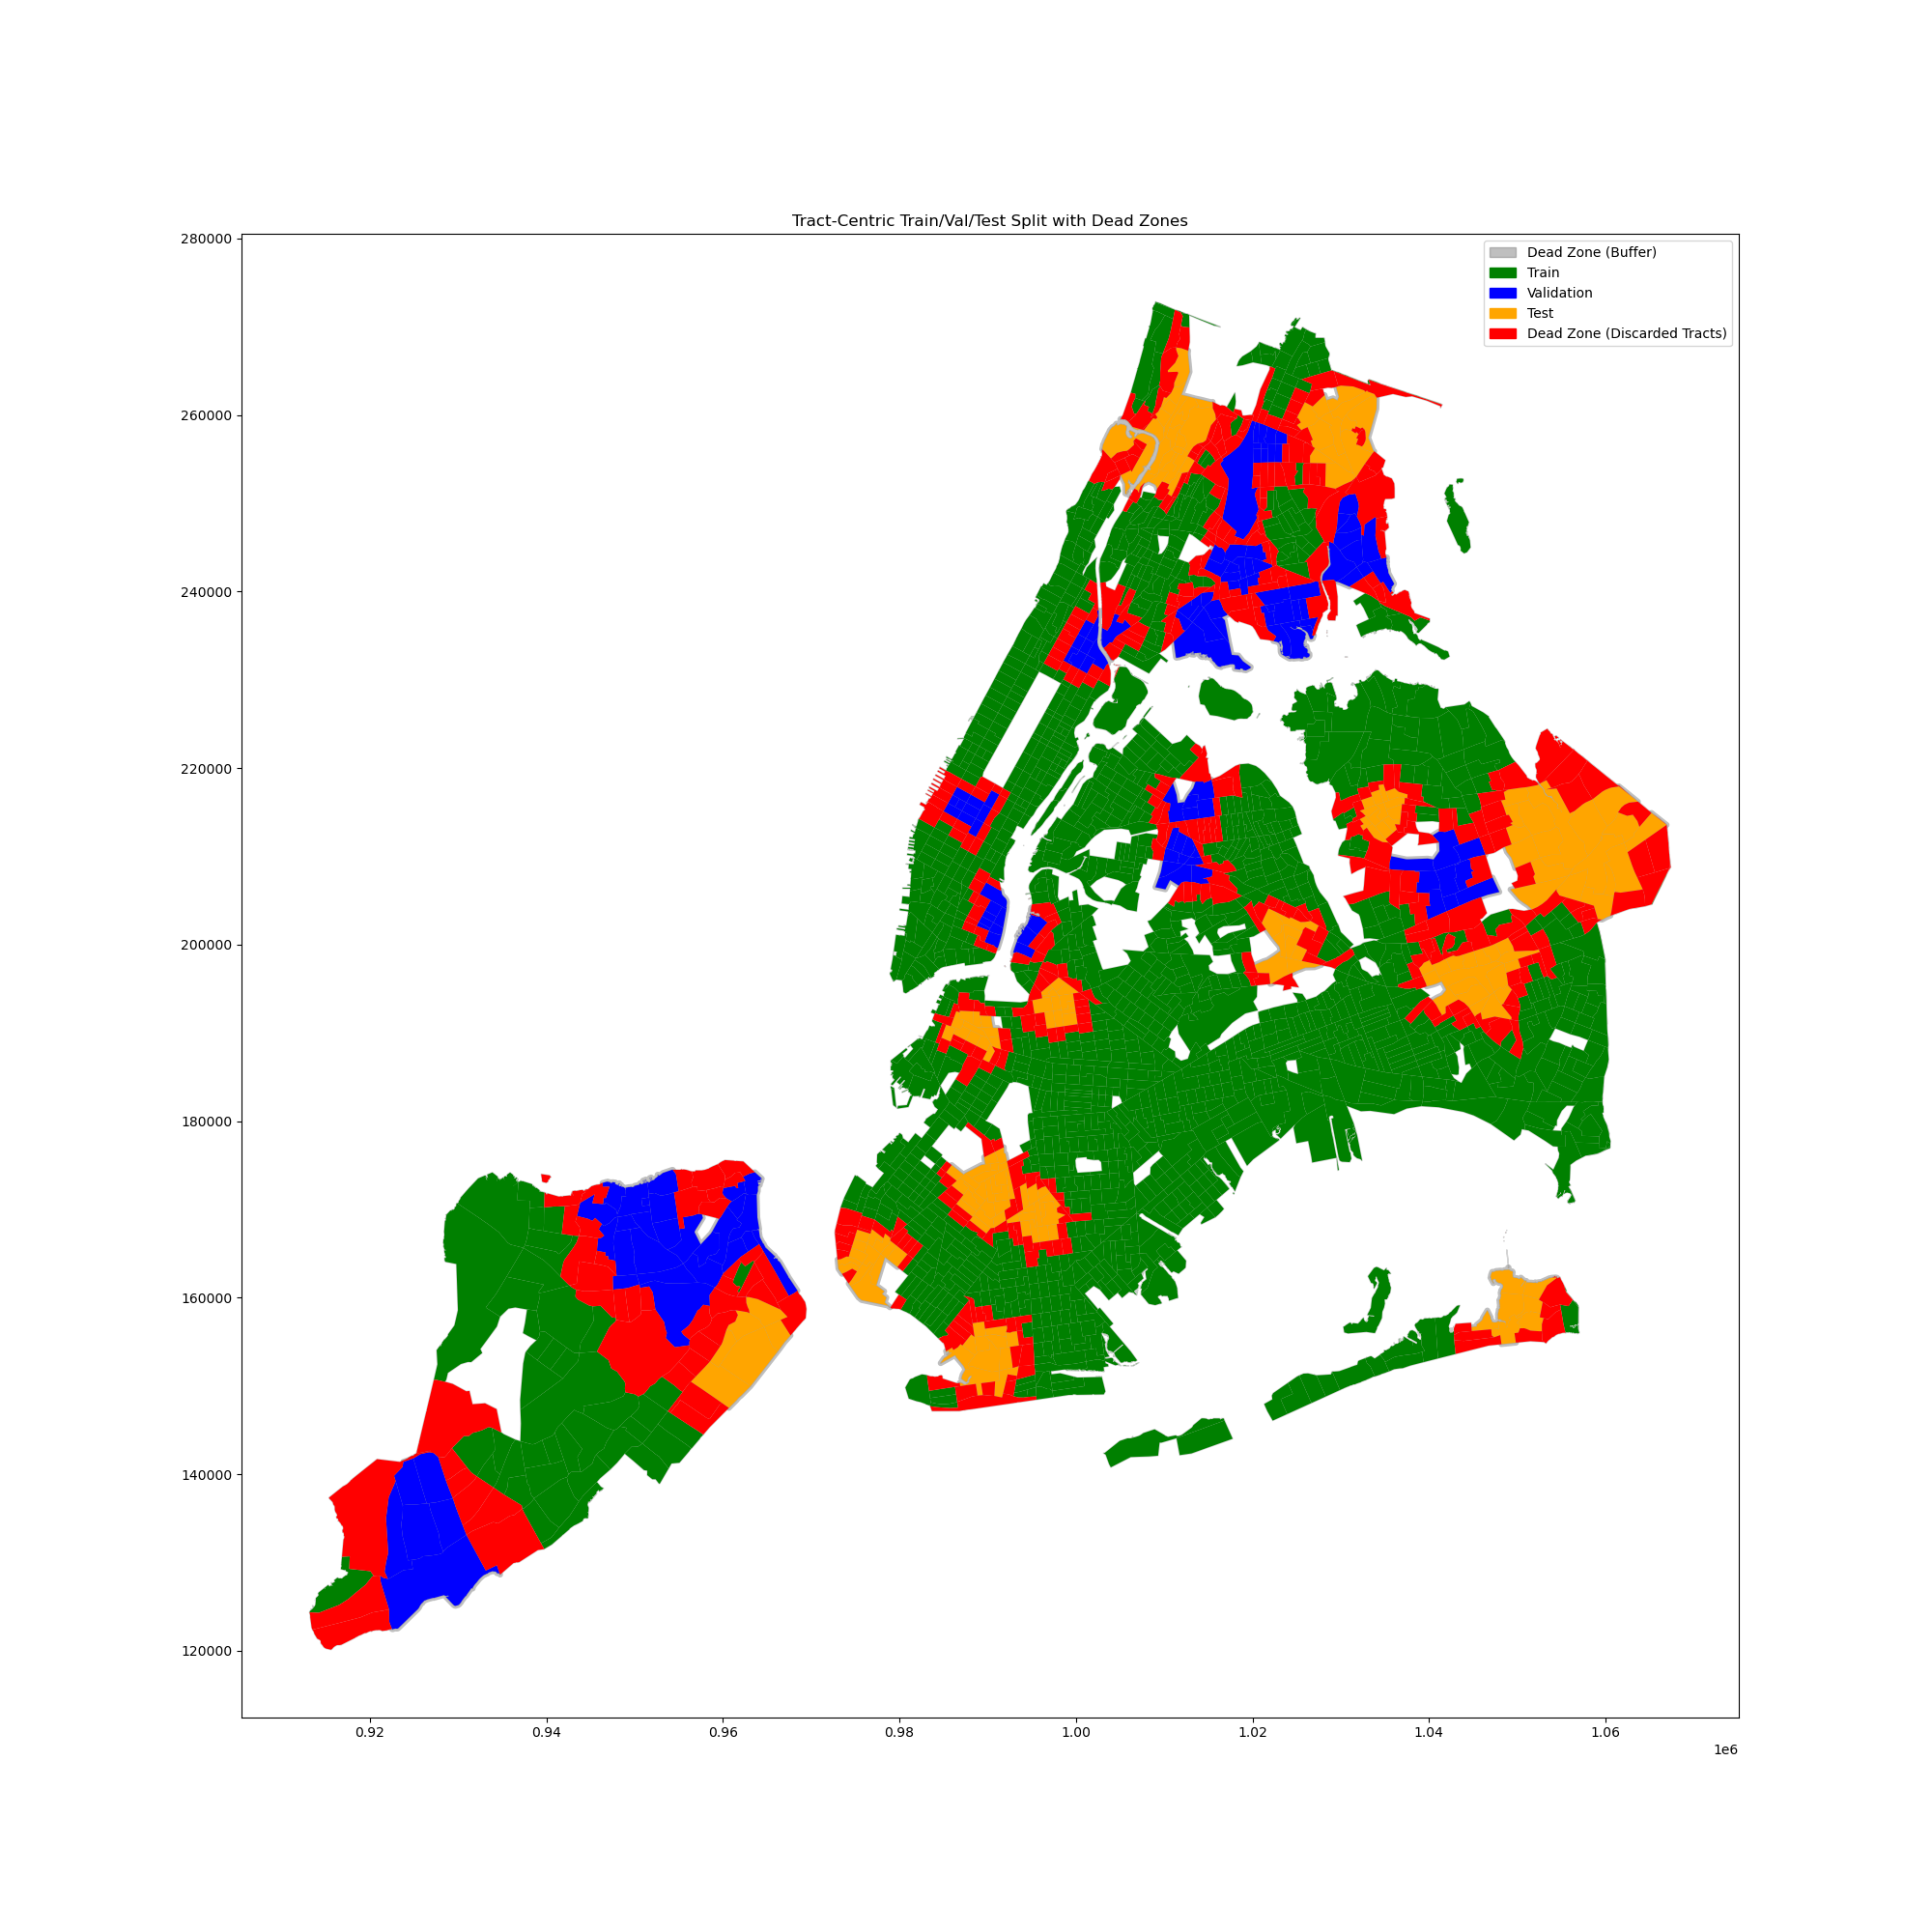
\includegraphics[width=\linewidth]{Figures/tract_splits_with_dead_zone.png}
    \caption{Census tract partition: train (blue), test (red), validation (green), and dead-zone buffer (grey). Test tracts form geographically compact, income-stratified clusters. The dead zone prevents training tiles from capturing visual context from within test-tract boundaries.}
    \label{fig:splits}
\end{figure}

Training uses AdamW with initial learning rate $10^{-4}$ and a ReduceLROnPlateau schedule (decay factor 0.8, patience 20 epochs, floor at $\mathrm{lr}/20$). Gradients are accumulated over 8 micro-batches before each optimizer step (physical batch size 8; effective batch size 64 cross-sectional images per update). The temporal change ranking loss $\mathcal{L}_{change}$ is disabled in this implementation (the batch sampler draws only stable temporal twins); it is retained in the architecture for future use when a larger training set of verified structurally-changed buildings is available.

\subsection{Model Architecture and Training}
\label{sec:model}

At its core, the model takes as input an aerial image tile centered on a building footprint---together with a set of geographic covariates---and produces a single scalar score representing that building's relative structural wealth position at a given point in time. The full pipeline then aggregates these building-level scores to the census tract, maps their empirical quantiles to a target income distribution, and delivers zero-shot econometric estimates for any city without requiring additional labeled data.

The architecture is designed around a \textbf{dual objective}. First, it learns a monotonic ordinal continuum: the scalar score must strictly preserve the cross-sectional wealth ranking of buildings within a city at any given point in time. Second, it enforces temporal consistency: a physically stable building should occupy an invariant position on that continuum regardless of the year of observation, while a building that undergoes structural transformation should be displaced accordingly. Achieving both objectives simultaneously requires careful attention to which comparisons are econometrically valid.

% \paragraph{The comparability constraint.}
% This theoretical interpretation disciplines which comparisons the model may learn from. The network is a deterministic function of the image tile and its covariates. Given the same physical structure and the same local environment, it must produce the same score---this is not merely a desirable property but a logical consequence of the human wealth interpretation: a stable building in an unchanged neighborhood represents the same latent wealth bundle across time, so its mapping must be invariant. This gives rise to a strict comparability constraint on valid training pairs.

% Two observations of the same building at different times---$(b, i, t)$ and $(b, i, t')$---are \textit{directly comparable}. If no structural change has occurred, the human wealth bundle is identical and the scores should agree; if change has occurred, the displacement in score space is identified by the change in the bundle itself. Two different buildings observed in the \textit{same} year---$(b, i, t)$ and $(c, j, t)$---are also \textit{directly comparable}, since both are positioned within the same city-wide income distribution at the same moment in time and the cross-sectional ordering is well-defined.

% However, supervising the network with direct ACS label comparisons across \textit{both} dimensions simultaneously---$(b, i, t)$ against $(c, j, t')$ for $b \neq c$ and $t \neq t'$---is empirically unidentified. While Lemma 1 of our Representation Theorem guarantees that a true cross-spatiotemporal ordering exists in the latent wealth space, the observed ACS income distributions drift aggregately over time. A naive comparison of ACS labels across different buildings and different years conflates the true spatial wealth gradient with aggregate temporal drift. Therefore, the in-batch pairwise framework strictly masks out spatiotemporal pairs during training. The network is forced to \textit{learn} the cross-spatiotemporal bridge (Lemma 1) endogenously, by chaining together valid cross-sectional and temporal-trajectory gradients, rather than anchoring to historically drifted labels.

To enforce these objectives without introducing spatial cardinality mismatch or temporal label drift, we adopt an \textbf{In-Batch Pairwise Ranking} framework and abandon cardinal regression entirely. The loss supervises only the \textit{direction} of pairwise score differences, never their magnitude. This resolves the label-inconsistency problem inherent in longitudinal ACS data. By supervising direction alone, the model learns a transport function that connects how buildings behave over time without anchoring to historically corrupted magnitudes.

% \subsubsection{Image Input and Spatial Spillover ($\tau$)}

% Building footprint polygons are sourced from the official New York City Department of Information Technology and Telecommunications (DoITT) dataset. These polygons are used exclusively to identify building centroids; the polygon geometry itself is never fed to the network. Instead, for each building $b$, the model receives a raw multi-spectral aerial image tile centered on the building's centroid.

% Because neighborhood wealth is shaped by localized externalities that extend beyond any single structure, the image tile is not clipped to the building footprint. We introduce a \textbf{spatial spillover hyperparameter, $\tau$}, defined as a buffer radius (in meters) around the centroid, so that the tile captures the immediate built environment surrounding the building. Let $X_{b,i,t}^\tau$ denote the aerial image tile of building $b$ in tract $i$ at year $t \in \{2008, 2010, 2012, 2014, 2016, 2018, 2020, 2022, 2024\}$, inclusive of the $\tau$-meter buffer.



\subsubsection{Feature Extraction: ScaleMAE with Low-Rank Adaptation}

The feature extractor is a \textbf{ScaleMAE} (Scale-aware Masked Autoencoder) backbone \citep{reed2023scalemae}, a Vision Transformer (ViT-Large/16) pretrained on multi-scale remote sensing imagery via masked image modeling. ScaleMAE is specifically designed to encode spatial resolution as a learned positional signal, making it well-suited for aerial imagery where the ground sampling distance (GSD) varies across acquisitions and zoom levels.

To adapt the pretrained backbone to the ordinal ranking task without catastrophic forgetting, we apply \textbf{Low-Rank Adaptation (LoRA)} \citep{hu2021lora} to the attention and MLP projection matrices of every transformer block. Specifically, trainable low-rank decomposition matrices of rank $r = 16$ are injected into the fused query-key-value attention projections (\texttt{qkv}) and the two MLP layers (\texttt{fc1}, \texttt{fc2}) of each block. The original pretrained weights remain frozen; only the LoRA adapters and the downstream regression head are updated during training. This reduces the trainable parameter count by over 99\% relative to full fine-tuning while preserving the rich spatial representations learned during pretraining.

The ScaleMAE backbone encodes each image tile from building $b$ in tract $i$ at year $t$, $X_{b,i,t}^\tau$ into a sequence of patch token embeddings. Mean-pooling across the spatial patch dimension yields a single feature vector:
\begin{equation}
h_{b,i,t} = \text{MeanPool}\!\left( f_\theta\!\left(X_{b,i,t}^\tau\right) \right) \in \mathbb{R}^{1024}
\end{equation}
where $f_\theta$ denotes the LoRA-augmented ScaleMAE backbone.

\subsubsection{Late Fusion Score Head}

A \textbf{Late Fusion Head} projects the pooled image embedding---concatenated with an optional geographic covariate vector---onto a single scalar score. The architecture consists of:
\begin{enumerate}
    \item A linear compression layer that maps the 1024-dimensional image embedding to 64 dimensions, followed by GELU activation, layer normalization, and 40\% dropout.
    \item A final linear layer that maps the concatenation of the 64-dimensional compressed image features and the metadata vector $\mathbf{m}_{b,i,t}$ (\textbf{currently a single covariate: distance-to-city-center}) to the scalar output.
\end{enumerate}

The scalar output is:
\begin{equation}
\hat{R}_{b,i,t} = g_\phi\!\left(h_{b,i,t},\; \mathbf{m}_{b,i,t}\right)
\end{equation}
where $g_\phi$ denotes the late fusion head with weights $\phi$.

This scalar $\hat{R}_{b,i,t}$ represents the building's position on the ordinal poor-to-rich continuum. Within a census tract $i$, buildings share the same underlying socioeconomic context, so in expectation, $E_i \hat{R}_{b,i,t} = \hat{R}_{i,t}$ for all $b$. Deviations across buildings within the same tract are treated as measurement error. Because the model is never fed more than a few buildings per tract per epoch, it is regularized against overfitting to the visual idiosyncrasies of individual structures and is instead forced to learn the structural hierarchy of wealth at the neighborhood level.

\subsubsection{Batch Construction and Sampling Strategy}

The training pipeline constructs stochastically stratified \textbf{hybrid batches}, each designed to maximize pairwise supervision density from a single unified forward pass through the backbone.

\paragraph{The Cross-Sectional Core ($\mathcal{B}_{cs}$)}
A \texttt{HybridBatchSampler} randomly selects a single anchor year $t$ and draws $B_{cs}$ distinct buildings from different census tracts observed in that year. This cross-sectional core is the primary source of ordinal ranking supervision: every unique pair of buildings from different census tracts provides a valid directional constraint.

\paragraph{The Temporal Auxiliary Set ($\mathcal{B}_{temp}$)}
For a fraction of the buildings in $\mathcal{B}_{cs}$ (controlled by the hyperparameter $\rho_{temp}$, default 0.20), the sampler queries the longitudinal panel for observations of the same building in a different year $t' \neq t$:
\begin{itemize}
    \item \textbf{Stable twins:} If building $k$ exists in $t'$ and underwent no structural change ($I_{k}^{valid}(t \to t') = 0$), the image for $t'$ is appended to the batch, contributing to the temporal stability penalty.
    \item \textbf{Changed twins:} If building $k$ exists in $t'$ but underwent statistically significant structural change ($I_{k}^{valid}(t \to t') = 1$), the image for $t'$ is appended to the batch, contributing to the temporal change ranking objective.
\end{itemize}

\noindent The complete hybrid batch is therefore $\mathcal{B} = \mathcal{B}_{cs} \cup \mathcal{B}_{temp}$, processed in a \textit{single forward pass} through the shared backbone.

\subsubsection{Loss function}

A single forward pass encodes the entire hybrid batch $\mathcal{B}$ into a vector of scalar scores $\hat{R}$. The total loss is the decoupled sum of three objectives computed over valid subsets of these scores, plus a variance regularizer that prevents score collapse.

\paragraph{Cross-Sectional Ranking ($\mathcal{L}_{cross}$)}

% For the $B_{cs}$ cross-sectional images in year $t$, we enumerate all $\binom{B_{cs}}{2}$ unique, undirected pairs via the upper-triangular indices. Let $\mathcal{U}_{valid}$ denote the subset of unique pairs $(k, l)$ where buildings $k$ and $l$ reside in \textit{different} census tracts (same-tract pairs are masked out, as ACS labels provide no intra-tract variation).

Let $y_{k,l} = \text{sign}(Z_l - Z_k) \in \{-1, +1\}$ denote the true economic ordering from ACS labels, where $Z$ is the label (relative income score). We define the signed agreement as $\delta_{k,l} = y_{k,l} \cdot (\hat{R}_l - \hat{R}_k)$, which is positive when the model's ranking agrees with the ground truth.

The cross-sectional loss uses a \textbf{smooth logistic (RankNet) surrogate}:
\begin{equation}
\mathcal{L}_{cross} = \frac{1}{|\mathcal{U}_{valid}|} \sum_{(k,l) \in \mathcal{U}_{valid}} \log\!\left(1 + \exp\!\left(-\frac{\delta_{k,l}}{T}\right)\right)
\end{equation}
where $T$ is a temperature parameter that controls the sharpness of the logistic sigmoid.\footnote{The temperature paramenter $T$ is set to 1. A fixed temperature is sufficient because the variance regularizer $\mathcal{L}_{var}$ independently anchors the standard deviation of cross-sectional scores to 1.0 throughout training, keeping the effective gradient scale stable without requiring $T$ to adapt to $\sigma_{batch}$. This design preserves the ordinal framework: supervision is purely directional (sign of label differences), and $T$ merely controls the gradient sharpness around the decision boundary without injecting cardinal economic content.}

\paragraph{Temporal Stability Penalty ($\mathcal{L}_{stable}$)}

For buildings in the stable temporal subset $\mathcal{B}_{stable}$, the latent human wealth bundle is physically identical between years $t$ and $t'$. The model enforces temporal invariance via a mean squared error (L2) penalty. Each temporal twin is dynamically paired with its cross-sectional anchor by matching on building identifier (DOITT\_ID):
\begin{equation}
\mathcal{L}_{stable} = \frac{1}{|\mathcal{B}_{stable}|} \sum_{k \in \mathcal{B}_{stable}} \left( \hat{R}_{k,t} - \hat{R}_{k,t'} \right)^2
\end{equation}

% \paragraph{Temporal Change Ranking ($\mathcal{L}_{change}$)}

% For buildings in the changed temporal subset $\mathcal{B}_{change}$, physical alteration identifies a shift in the human wealth bundle. Let $y_{k, t \to t'} \in \{-1, +1\}$ indicate the direction of the structural change (e.g., $+1$ if the tract gentrified). We supervise this displacement using the same smooth logistic surrogate used for cross-sectional ranking, applied to temporal pairs of the \textit{same} building:
% \begin{equation}
% \mathcal{L}_{change} = \frac{1}{|\mathcal{B}_{change}|} \sum_{k \in \mathcal{B}_{change}} \log\!\left(1 + \exp\!\left(-\frac{y_{k,t\to t'} \cdot (\hat{R}_{k,t'} - \hat{R}_{k,t})}{T_{change}}\right)\right)
% \end{equation}
% where $T_{change} = m_{base}$, consistent with the fixed temperature used for cross-sectional ranking.

\paragraph{Variance Regularizer}

To prevent the score head from collapsing its output to a near-constant value---a failure mode in which the softplus loss can be trivially minimized by shrinking $\sigma_{batch}$ toward zero---we add a quadratic variance penalty computed exclusively over the cross-sectional scores:
\begin{equation}
\mathcal{L}_{var} = \left(\sigma_{cs} - 1\right)^2
\end{equation}
where $\sigma_{cs} = \text{std}(\hat{R}_{cs})$. This targets a unit standard deviation for the cross-sectional score distribution, ensuring the model maintains a well-spread prediction landscape. The penalty is applied only to cross-sectional scores (not temporal), maintaining internal consistency: both the temperature $T$ and the variance target reference the same $\sigma_{cs}$, eliminating any tug-of-war between temporal invariance and score spread.

\paragraph{Total Objective}

The final unified objective aggregates the valid comparisons:
\begin{equation}
\mathcal{L}_{total} = \mathcal{L}_{cross} + \lambda_{s} \cdot \mathcal{L}_{stable} + \mathcal{L}_{var} %+ \lambda_{c} \cdot \mathcal{L}_{change}
\end{equation}
where $\lambda_s$ is the weighting hyperparameter governing the relative influence of the temporal constraints against the cross-sectional ranking baseline.

% \paragraph{Relation to the literature.} The cross-sectional ranking component of the loss is a smooth logistic pairwise surrogate, structurally identical to the RankNet formulation of \citet{burges2005learning}. The logistic surrogate is preferred over the hard hinge variant of \citet{joachims2002optimizing} because the smooth gradient propagates useful learning signal even for correctly ranked pairs, avoiding the dead-zone problem inherent in hinge losses where gradients vanish for pairs satisfying the margin constraint. The use of a fixed temperature $T = m_{base}$ decoupled from label magnitudes—with score-spread control delegated entirely to the variance regularizer $\mathcal{L}_{var}$—is, to our knowledge, novel in the satellite-imagery-for-economics literature. The combination of an unconditional L1 stability penalty on temporal positives with a directional logistic surrogate on negatives is structurally analogous to the Large Margin Nearest Neighbor objective of \citet{weinberger2009distance}, adapted from metric space to a 1-D scalar continuum. The curriculum learning schedule over quintile-based pair difficulty draws on the general curriculum learning framework of \citet{bengio2009curriculum}. To our knowledge, this specific combination---smooth ordinal supervision with score-based adaptive temperature, stable temporal anchors, directional structural change indicators, and progressive pair-difficulty curriculum---has not been applied previously in the satellite-imagery-for-economics literature, where existing work relies on cross-sectional regression \citep{jean2016combining} or cardinal pairwise differences \citep{yeh2020using} rather than a purely ordinal framework.

\subsubsection{Curriculum learning: easy-to-hard pair filtering.}
To improve gradient quality and prevent the model from fitting to noisy, ambiguous comparisons early in training, we implement an epoch-dependent curriculum that progressively admits harder pairwise comparisons. Each building is assigned to a score quintile bin $q \in \{1, 2, 3, 4, 5\}$ based on its ACS label. The absolute bin difference $|q_k - q_l|$ between paired buildings determines the difficulty of the comparison: large differences correspond to ``easy'' pairs with unambiguous ordinal direction, while small differences correspond to ``hard'' pairs where ACS measurement error may reverse the true ordering.

The curriculum schedule is:
\begin{itemize}
    \item \textbf{Epochs 0--59:} Only pairs with $|q_k - q_l| \geq 3$ (extreme quintile contrasts).
    \item \textbf{Epochs 60--149:} Pairs with $|q_k - q_l| \geq 2$ (adjacent quintile pairs admitted).
    \item \textbf{Epoch 150+:} Pairs with $|q_k - q_l| \geq 1$ (all inter-quintile pairs admitted).
\end{itemize}
Intra-quintile comparisons ($|q_k - q_l| = 0$) are \textit{permanently excluded}. The ACS margin of error makes within-quintile rankings pure noise; forcing a strict directional constraint on such pairs causes variance collapse as the model learns to shrink its output spread to trivially satisfy the loss.


\subsubsection{Out-of-Sample Generalizability and Quantile Mapping}

A core methodological commitment of this architecture is the intentional discarding of spatial cardinality at every stage of training and deployment. Urban morphologies scale differently: a one-standard-deviation increase in structural wealth in New York City manifests vertically, in building height and facade quality, whereas in Dallas the same gradient manifests horizontally, in lot size and setback. A model that learns absolute topological anchors from one city's training data will not transfer cleanly to another. By constraining the network to act as a pure monotonic ordinal ranker, we decouple the learned embedding from city-specific scaling.

Deployment to recover the absolute wealth rankings proceeds as follows. The model computes scalar scores $\hat{R}$ for all target buildings based solely on their aerial imagery. Empirical quantiles of these scores are then mapped directly to the corresponding quantiles of the target city's ACS income distribution, delivering zero-shot econometric moment matching without any fine-tuning on labeled local data.

% \subsubsection{Training Infrastructure}

% \paragraph{Cyclic cache management.}
% Because the full panel of aerial imagery for New York City exceeds available RAM, the training pipeline employs a \textbf{cyclic cache manager} that maintains a rotating window of pre-extracted, subsampled image shards on disk. Training proceeds over a fixed number of active shards; while the GPU processes the current shards, a background thread asynchronously generates the next batch of shards from the zarr-backed imagery store. This ensures the GPU is never starved for data while keeping RAM usage bounded.

% \paragraph{Mixed-precision training and gradient accumulation.}
% All forward passes are executed under \textbf{automatic mixed precision} (AMP) with float16 compute and float32 master weights, managed by a \texttt{GradScaler}. To achieve an effective batch size larger than the physical GPU memory allows, gradients are accumulated over $K$ micro-batches (default $K = 8$) before each optimizer step. This is equivalent to training with an effective batch of $B_{cs} \times K$ cross-sectional images, dramatically increasing the number of valid pairwise constraints per parameter update.

% \paragraph{Optimizer and learning rate schedule.}
% The optimizer is AdamW with weight decay 0.05. The learning rate follows a \textbf{ReduceLROnPlateau} schedule that monitors mean validation Spearman correlation, decaying by a factor of 0.8 after 20 epochs of no improvement, with a minimum learning rate floor of $\text{lr}/20$.

% \paragraph{Data augmentation.}
% Training tiles are extracted with a jitter pad of $\pm 10$ meters around the centroid, which is then realized as a random spatial crop at model resolution. Photometric augmentations include color jitter (brightness $\pm 0.3$, contrast $\pm 0.3$, saturation $\pm 0.2$), random grayscale (10\%), random horizontal and vertical flips. Validation and inference tiles receive no augmentation beyond ImageNet normalization.

% \paragraph{Validation metric.}
% Validation is performed using pointwise MSE loss for interpretable per-image tracking, complemented by \textbf{Spearman rank correlation} between predicted scores and ACS labels as the primary model selection criterion. The best model checkpoint is selected to maximize mean Spearman correlation across validation splits.

\subsubsection*{Summary of Core Architectural Hyperparameters (Runtime Values)}
\begin{itemize}
    \item \textbf{$\tau$ (Spillover Radius):} Buffer radius (in meters) around the building centroid defining the spatial extent of each aerial image tile. Value: 100\,m.
    \item \textbf{$\rho_{temp}$ (Temporal Fraction):} Fraction of the batch reserved for temporal auxiliary images (stable twins only in current implementation). Value: 0.40.
    % \item \textbf{$m_{base}$ (Fixed Temperature):} The temperature $T = m_{base}$ used in the logistic ranking surrogate. Value: 1.0.
    \item \textbf{$\lambda_s$ (Stable Temporal Weight):} Weighting of the temporal stability L2 penalty. Value: 0.3.
    \item \textbf{$\lambda_c$ (Change Temporal Weight):} Weighting of the temporal change ranking loss. Effectively 0 in current training (sampler draws only stable twins).
\end{itemize}

\section{Results}\label{sec:results}

\begin{figure*}
    \centering
    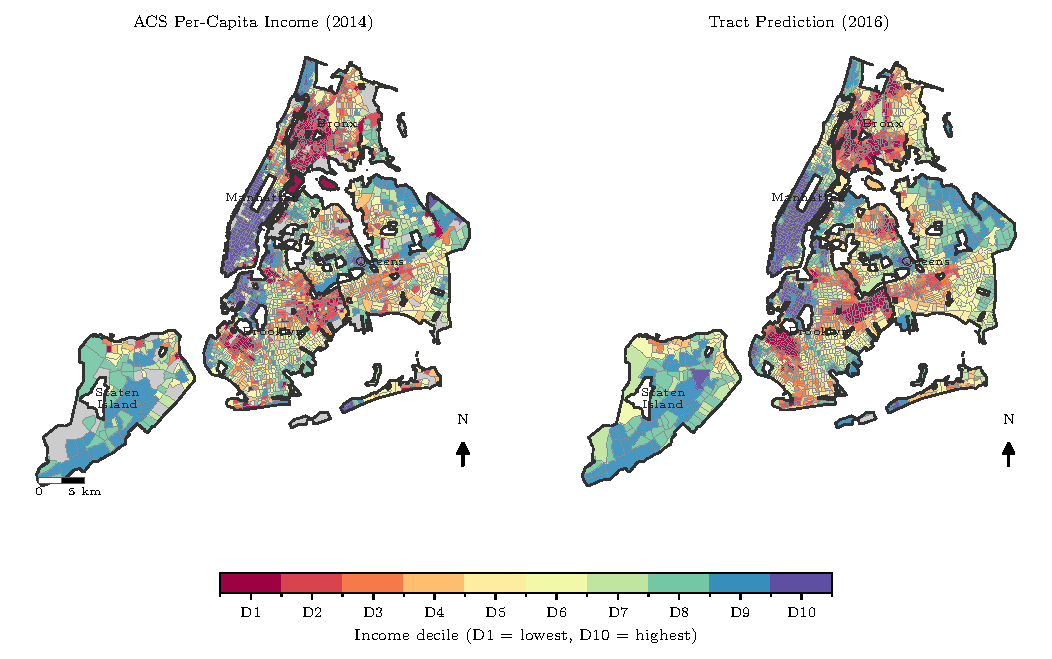
\includegraphics[width=\linewidth]{Figures/A_map_acs2014_pred2016.pdf}
    \caption{Comparison of ACS per-capita income deciles (2014) and tract-level model predictions (2016) across New York City. The left panel shows the ground-truth deciles from the American Community Survey, with missing survey data represented in grey. The right panel displays the model's aggregated predictions. Both maps share the income decile scale shown at the bottom, where D1 represents the lowest income decile and D10 represents the highest.}
    \label{fig:map}
\end{figure*}

\begin{figure*}
    \centering
    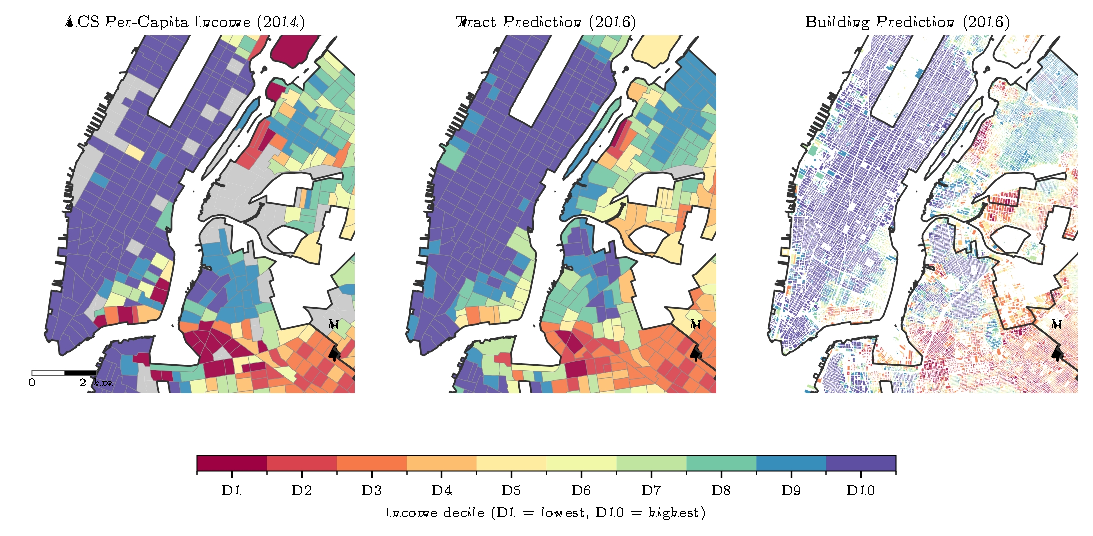
\includegraphics[width=\linewidth]{Figures/A_map_zoom_core.pdf}
    \caption{Comparison of tract-level and building-level predictions in Manhattan, Brooklyn and Queens. The left panel shows the 2014 ACS per-capita income deciles (with missing data in grey), the middle panel shows the aggregated 2016 tract-level model predictions, and the right panel displays the 2016 individual building-level predictions. The comparison highlights the model's capacity to resolve micro-spatial variations and sub-tract socio-economic heterogeneity.}
    \label{fig:map_zoom}
\end{figure*}


Evaluating this model is complicated by the absence of ground-truth income at the building level: the ACS reports averages for census tracts, not individual structures. We therefore organize the evaluation along the two dimensions the model is designed to capture—cross-sectional and longitudinal—each validated against the aggregation level at which a ground truth exists. We first assess \emph{cross-sectional} validity by aggregating building-level predictions to the tract level and comparing them against ACS relative income. Section~\ref{sec:results} (Model predictions) shows that the predicted spatial distribution reproduces known wealth patterns across the five boroughs while resolving within-tract heterogeneity that tract-level survey data cannot, and the cross-sectional scatter establishes that this holds in a tract-and-year combination withheld entirely from training. We then assess \emph{longitudinal} behavior, which a useful model must get right in two opposite ways: predictions for physically stable buildings should stay stable over time, while predictions for buildings undergoing genuine structural change should move. We test the first property directly through a temporal-consistency analysis—within-building variability, rank autocorrelation across years, and individual building trajectories—and the second through a Callaway--Sant'Anna event study that asks whether new construction shifts predicted scores. Finally, we map the ordinal scores onto local income quantiles to recover cardinal estimates, verifying that the resulting city-level moments and long-run changes track the ACS benchmark.

\subsection{Model predictions}
To illustrate the main output of the model, Figure \ref{fig:map} compares the spatial distribution of tract-aggregated model predictions for 2016 against the American Community Survey (ACS) per-capita income deciles from 2014. Geographically, there is a visible correspondence in broad wealth patterns across the five boroughs. Higher-income deciles (represented by blue and purple hues) are concentrated in Manhattan, while lower-income deciles (represented by red and orange hues) are clustered in parts of the Bronx and central Brooklyn. This overall alignment suggests that the ordinal model, despite being trained without cardinal income targets, identifies structural features in high-resolution aerial imagery that correlate reasonably well with ground-truth economic indicators at a macro scale.

To illustrate the model's capacity to resolve micro-spatial variation, Figure \ref{fig:map_zoom} zooms in on Manhattan and the adjacent Brooklyn waterfront and Queens neighborhood. The left and middle panels illustrate the structural limitations of tract-level representations: administrative boundaries average out localized economic disparities, and missing survey data (represented in grey) can obscure entire blocks. By contrast, the building-level predictions in the rightmost panel map out a highly granular spatial distribution. By resolving individual building footprints, the model identifies sharp socioeconomic transitions that are typically masked. Along the East River waterfront, for instance, high-income predictions (blue and purple) associated with newer, high-density residential developments are resolved directly adjacent to blocks with lower predicted scores (red and orange), highlighting localized wealth disparities that tract-level aggregations smooth over.


\subsection{Cross-Sectional Validity}

The visual correspondence in Figure~\ref{fig:map} is suggestive but informal. To test it rigorously, we quantify the agreement between predictions and survey income out-of-sample. Figure~\ref{fig:scatter2016} plots, for each census tract in the test set, the mean predicted score against the ACS Z-score for the year 2016. This comparison is doubly out-of-sample: test tracts are spatially separated from all training tracts (Section~\ref{sec:splits}), and 2016 imagery was entirely excluded from training (temporal holdout). The strong monotone relationship visible in the scatter---reinforced by the 10-bin conditional mean overlay---demonstrates that the model has learned feature representations generalizable both across space and across time. Quantitatively, the Spearman rank correlation between predicted scores and ACS Z-scores across the $\approx 190$ test tracts equals $\rho = 0.850$ ($95\%$ bootstrap CI: $[0.834, 0.863]$), and the Kendall $\tau = 0.665$ ($95\%$ bootstrap CI: $[0.649, 0.681]$). Both are highly significant ($p < 0.001$). Spatial interpolation in aerial data is non-trivial: neighborhood characteristics can change abruptly at borough or zoning boundaries, and imaging conditions (sun angle, seasonal vegetation, etc) differ across acquisition years. The fact that the model maintains ordinal accuracy in a year and area it has never seen is direct evidence of genuine structural learning rather than memorization.

\begin{figure}[h!]
    \centering
    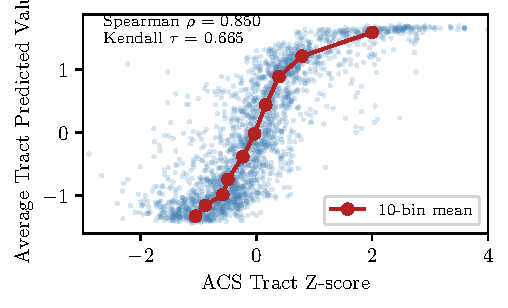
\includegraphics[width=\linewidth]{Figures/A_scatter_2016.pdf}
    \caption{Cross-sectional validity at the temporal holdout year (2016). Each dot is a test-set census tract. The horizontal axis is the ACS relative income Z-score; the vertical axis is the tract-averaged model prediction. The red line connects 10-decile conditional means. The test tracts are spatially isolated from all training data and 2016 imagery was not used in training, making this a joint spatial-and-temporal out-of-sample test.}
    \label{fig:scatter2016}
\end{figure}


\subsection{Longitudinal Consistency}

Cross-sectional accuracy establishes that the model reads wealth from a single image, but the central motivation of this paper is temporal. A longitudinal model must satisfy two opposing requirements: it must hold predictions steady for buildings that have not physically changed, and move them for buildings that have. We test the first property directly through a temporal-consistency analysis—within-building variability, rank autocorrelation across years, and individual building trajectories—and the second through a Callaway--Sant'Anna event study that asks whether new construction shifts predicted scores.

\subsubsection{Stability of predictions for unchanged buildings.}

\begin{table*}[htbp]
\centering
\begin{tabular}{lrrrrrr}
\toprule
\multirow{2}{*}{Set -- Trend}
  & \multirow{2}{*}{$N$}
  & \multicolumn{3}{c}{Within-Unit Std.\ Dev.}
  & \multirow{2}{*}{\makecell{Intraclass\\Correlation}}
  & \multirow{2}{*}{\makecell{Rank\\Autocorr.}} \\
\cmidrule(lr){3-5}
  & & Median & Q1 & Q3 & & \\
\midrule
Test  -- Stable  & 50{,}086 & 0.093 & 0.053 & 0.178 & 0.961 & 0.939 \\
Train -- Stable  & 25{,}125 & 0.078 & 0.043 & 0.144 & 0.971 & 0.958 \\
Test  -- Changed & 49{,}277 & 0.101 & 0.050 & 0.224 & 0.945 & 0.918 \\
Train -- Changed & 23{,}700 & 0.089 & 0.043 & 0.187 & 0.950 & 0.927 \\
\bottomrule
\end{tabular}
\caption{Building-level stability metrics by data split and trend group.
  Within-unit Std.\ Dev.\ is computed across each unit's observed years;
  ICC measures between-unit consistency; rank autocorrelation is the
  Spearman rank correlation between 2016 and 2024.}
\label{tab:metrics}
\end{table*}

Table~\ref{tab:metrics} reports within-building temporal variability for the test and train splits for building pairs between 2016 (test set year) and 2024, separately for buildings classified as structurally stable and buildings near significant new construction. For stable test-set buildings ($n = 50{,}086$), the median within-building standard deviation of predicted scores across all eight observation years is $0.093$ score units, with an interquartile range of $[0.053, 0.178]$. The Intraclass Correlation Coefficient (ICC) of $0.961$ confirms that the majority of the total variance in predictions reflects between-building differences rather than within-building noise over time. The Spearman rank autocorrelation between 2016 and 2024 predictions---spanning eight years, with 2016 being a temporal holdout---is $0.939$ across 50,078 buildings. At the census-tract level, rank autocorrelation between 2016 and 2024 tract-mean predictions reaches $0.971$ across the 190 test tracts (Table~\ref{tab:metrics}). Buildings classified as structurally changed (near significant new construction) show moderately lower ICC ($0.945$ on the test set) and rank autocorrelation ($0.919$), consistent with the model capturing genuine variation near construction events rather than pure noise, while missing most of the reallocation changes.


% To illustrate, Figure~\ref{fig:bldgtrajectories} presents individual building trajectories for a sample of five stable and five changed test-set buildings. Stable buildings show flat predicted-score profiles across the eight observed years, confirming that the model does not introduce spurious temporal drift for structures that have not changed. Changed buildings (identified by proximity to significant new construction; the dashed vertical line marks the construction year) show discernible upward displacement in predictions after the construction event, consistent with the event-study results at the tract level.

% \begin{figure*}[htbp]
%     \centering
%     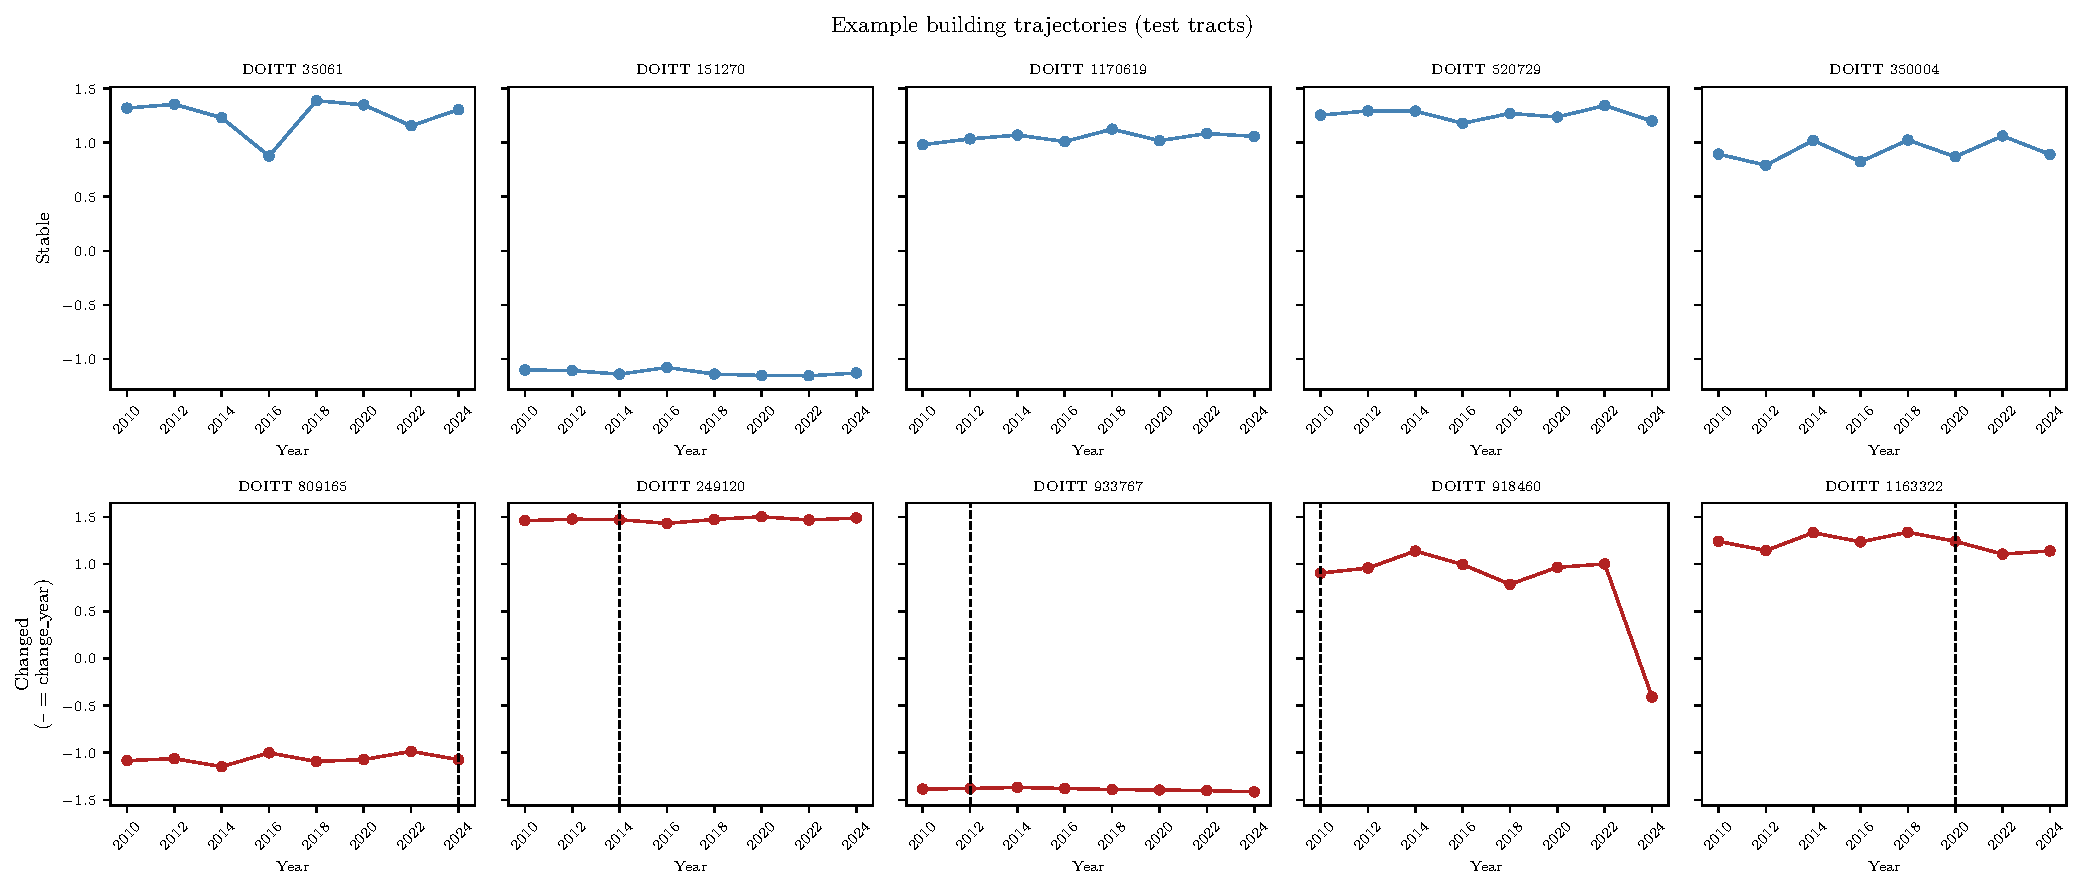
\includegraphics[width=\linewidth]{Figures/B_building_trajectories.pdf}
%     \caption{Example building-level prediction trajectories from test-set tracts. Top row: five randomly selected stable buildings. Bottom row: five buildings classified as changed (dashed vertical line marks construction year). Stable buildings show flat profiles; changed buildings show upward displacement around the construction event.}
%     \label{fig:bldgtrajectories}
% \end{figure*}


\subsubsection{Event study: new construction as a structural shock.}

Stability is only half of what a longitudinal model must deliver; the complement is responsiveness. We now test whether predictions move when neighborhoods physically change.

To formally test whether the model detects genuine structural improvements, we implement a Callaway and Sant'Anna \citep{callaway2021difference} staggered difference-in-differences at the census-tract level. The treatment is defined as the first year in which a tract's cumulative new building footprint area (buildings constructed 2010--2024) crosses a given percentage of its pre-2010 base footprint area. We consider three thresholds: 1\%, 5\%, and 10\%, capturing mild, moderate, and intensive construction activity. The outcome variable is the tract-level average model prediction (i.e., the mean ordinal score). Never-treated tracts serve as the control group.

Figure~\ref{fig:eventstudy} presents the event-time plots for both the test and train splits under each threshold. Pre-treatment trends are flat and centered near zero (normalized to the $k = -1$ reference period), supporting the parallel trends assumption. In this setup, the parallel trends assumption means that when no buildings changed, the predicted scores remain stable. After treatment, predicted scores rise significantly and persistently. The average treatment effect on the treated (ATT), aggregated across all post-treatment periods, is reported in Table~\ref{tab:csa}: the effect is statistically significant at all three thresholds and for both the test and train splits. Importantly, the ATT is monotonically increasing with the construction threshold---a tract where new construction represents 10\% of existing building area (ATT $\approx 0.14$ on the test set) shows substantially larger effects than one that barely crosses the 1\% threshold (ATT $\approx 0.04$).\footnote{Becuase the standard deviation of the predicted values is set to be 1, the ATT can be directly interpreted as an \textit{effect size}.} Further, the similarity between the effects for the test and train splits confirms that the model's responsiveness to structural change is not confined to the training distribution but generalizes to unseen areas. This dose-response pattern provides compelling evidence that the model's predictions are responsive to structural neighborhood change, not merely correlated with pre-existing trends, implying that the model is capturing genuine structural changes from the images. 

\begin{figure*}
    \centering
    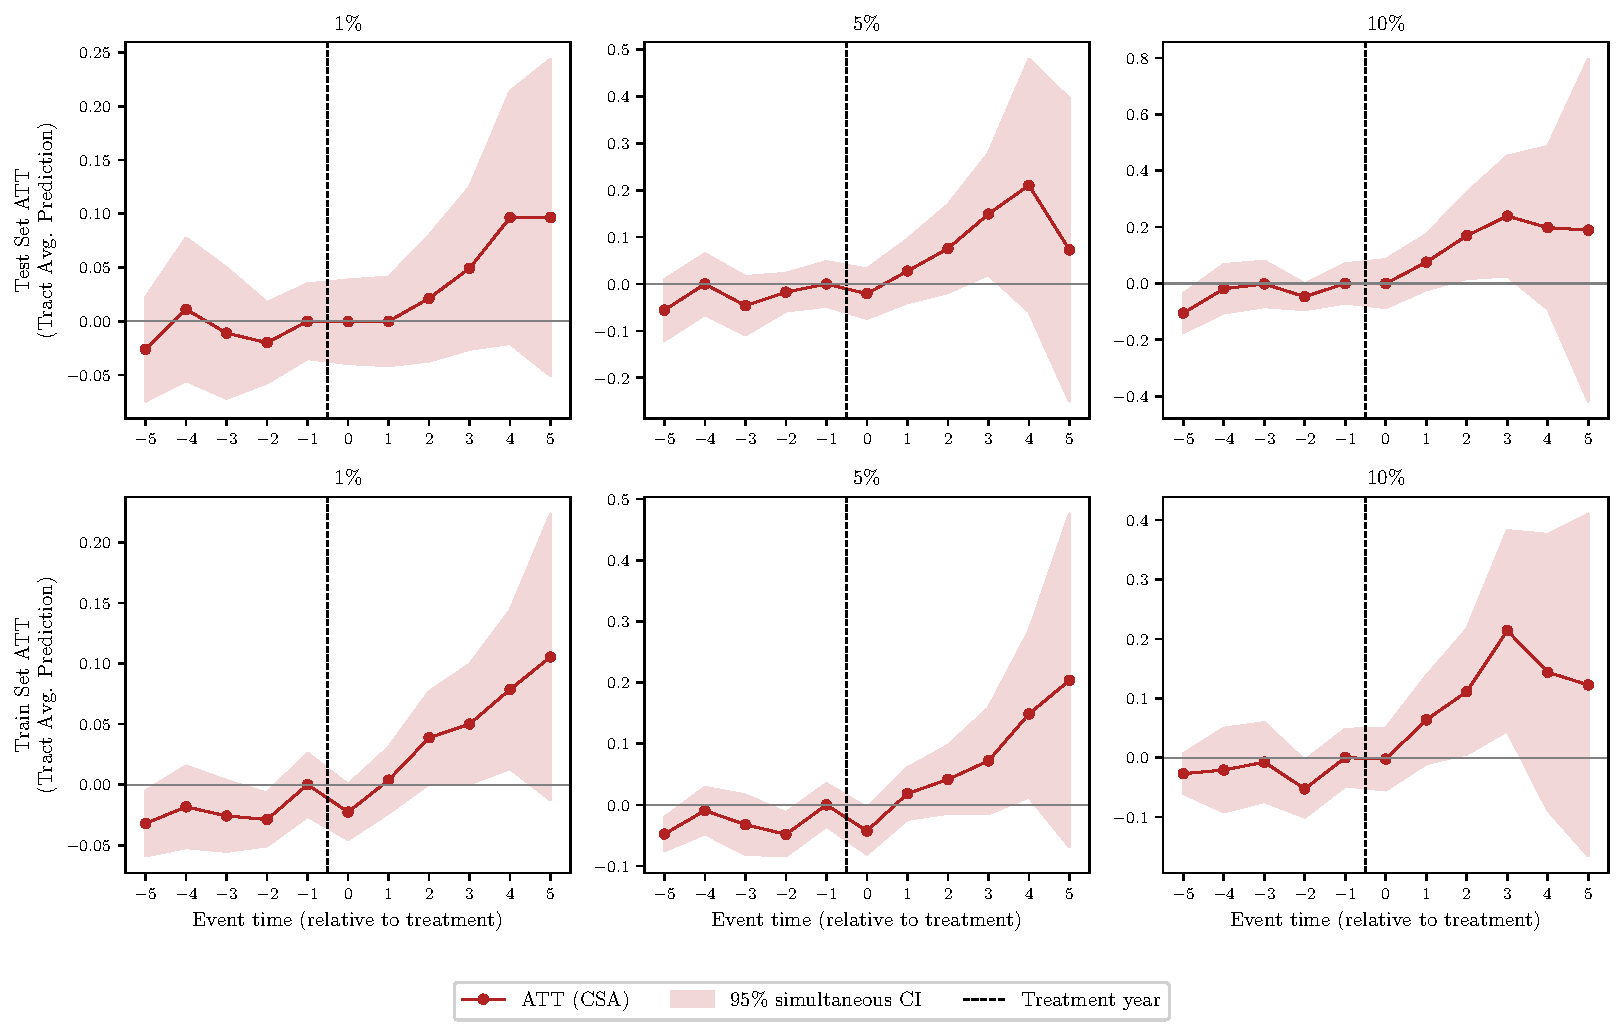
\includegraphics[width=\textwidth]{Figures/B_event_study_grid.pdf}
    \caption{Callaway--Sant'Anna event-study plots. Rows correspond to the test set (top) and train set (bottom). Columns correspond to construction intensity thresholds of 1\,\%, 5\,\%, and 10\,\% of pre-existing building footprint area. The horizontal axis is event time relative to the treatment year; the dashed vertical line marks the onset of treatment. ATTs and 95\,\% simultaneous bootstrap confidence bands are shown. Pre-treatment coefficients are normalized to $k = -1$.}
    \label{fig:eventstudy}
\end{figure*}

\begin{table}[htbp]
\centering
\begin{tabular}{lcc}
\toprule
\textbf{Threshold} & \textbf{Test ATT} & \textbf{Train ATT} \\
\midrule
1\%  & 0.0407\textsuperscript{*} & 0.0505\textsuperscript{*} \\
     & (0.0173)                  & (0.0109)                  \\
\addlinespace
5\%  & 0.0872\textsuperscript{*} & 0.0761\textsuperscript{*} \\
     & (0.0247)                  & (0.0159)                  \\
\addlinespace
10\% & 0.1439\textsuperscript{*} & 0.1232\textsuperscript{*} \\
     & (0.0342)                  & (0.0249)                  \\
\bottomrule
\multicolumn{3}{l}{\footnotesize \textsuperscript{*} Significant based on 95\% confidence band.} \\
\end{tabular}
\caption{Average Treatment Effect on the Treated (ATT) by Threshold and Split}
\label{tab:att_summary_se}
\end{table}


\subsection{City-average trajectory.}\label{sec:cardinal}
The preceding results validate the ordinal scores both cross-sectionally and over time. We now convert them into cardinal income estimates, which is what makes the predictions usable as a survey substitute.

To convert the dimensionless ordinal scores into cardinal income estimates, we apply a parametric quantile mapping. For each year $t$, we fit a Generalized Beta of the Second Kind (GB2) distribution \citep{mcdonald1984} by maximum likelihood to the ACS per-capita income distribution of all NYC census tracts. The GB2 is well-suited for income distributions because it has a power-law right tail and nests several commonly used income distributions (Dagum, Singh-Maddala, log-normal) as special cases. GB2 parameters are smoothed across years in log-space via a degree-3 polynomial to guard against MLE instability in any single year. Predicted scores are then mapped to the target distribution via empirical quantile-to-quantile matching: the rank of each building in the predicted score distribution is assigned the corresponding GB2 quantile. This procedure is rank-preserving by construction (Spearman correlation between raw scores and mapped values equals 1.0) and delivers city-level moments (mean income, variance) that are mechanically consistent with the ACS target.

Figure~\ref{fig:cityavg} plots the city-average mapped income trajectory alongside the ACS benchmark. The aggregate trajectory correctly reflects input moments, confirming that the distribution mapping is working as intended. \textbf{[TODO]} We could also add several economic indicators here like GINI, 90/10 ratio, etc, to confirm that the distribution mapping is not only reproducing the mean but also the shape of the target distribution. 

% \textbf{TODO: Generalization to another city.} The architecture is designed for zero-shot out-of-sample deployment: compute scores for any target city's buildings, empirical-quantile-map to local ACS moments. A validation on a second US city (e.g., Chicago or Los Angeles) would strengthen external validity claims. This test is currently pending due to data availability.

\begin{figure}[htbp]
    \centering
    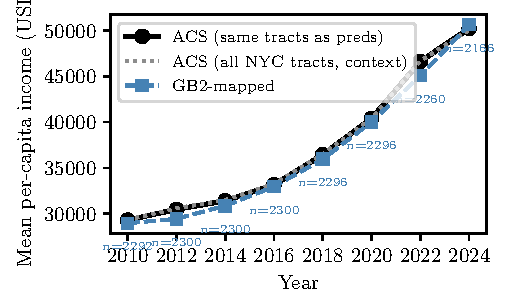
\includegraphics[width=\linewidth]{Figures/C_city_avg_trajectory.pdf}
    \caption{City-average trajectory. Black solid line: ACS mean per-capita income for the same census tracts with model predictions. Dashed line: ACS mean for all NYC tracts (context). Blue squares: GB2-mapped model predictions. Annotations show the number of predicted tracts per year.}
    \label{fig:cityavg}
\end{figure}

% \begin{figure}[htbp]
%     \centering
%     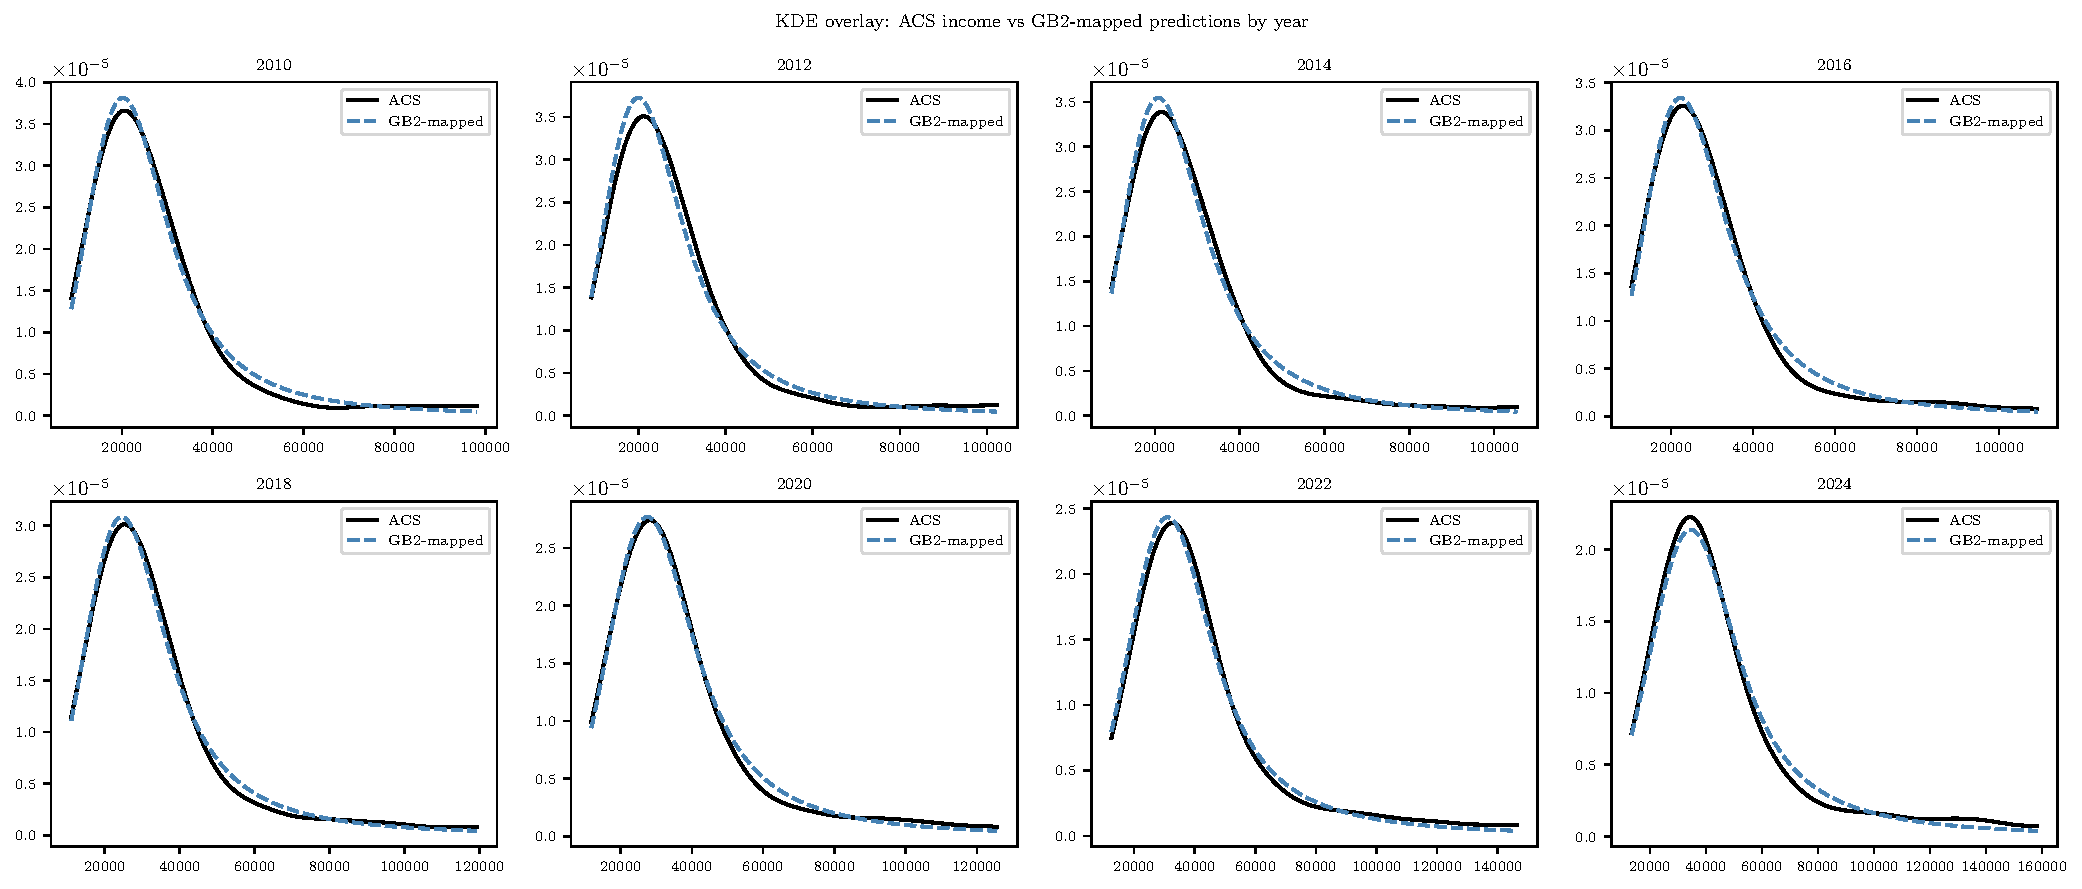
\includegraphics[width=\linewidth]{Figures/C_gb2_density_overlay.pdf}
%     \caption{Kernel density overlay of ACS income distribution (black) versus GB2-mapped model predictions (blue dashed) for each available year. Alignment confirms that the distribution mapping reproduces the shape, not just the mean, of the target distribution.}
%     \label{fig:gbdensity}
% \end{figure}

\subsection{Long-difference correlation. \textbf{The Weakness (for now!)}}

The city-average trajectory confirms that mapped \emph{levels} track the survey. A stronger test is whether mapped \emph{changes} do.


Figure~\ref{fig:longdiff} shows a long-difference scatter for tracts with both 2010 and 2024 model predictions (after GB2 distribution mapping to USD; see Section~\ref{sec:cardinal}): the horizontal axis plots the ACS per-capita income change from 2009 to 2024, and the vertical axis plots the corresponding change in mapped model predictions. The correlation is positive and significant but modest. This result is fully expected: the model is trained on purely visual, structural information and has no access to time-varying economic covariates such as educational attainment or industry composition. Gentrification or income growth driven by demographic sorting---without accompanying physical construction---is inherently invisible to the model. Nevertheless, the performance is still remarkable given the constraints: the spearman coefficient of $\rho=0.615$ confirms that the model's predictions are directionally consistent with true income changes, even if it cannot capture all the variation in those changes. \textbf{[TODO]} Adding time-varying ACS covariates (e.g., educational attainment, occupation structure) as auxiliary inputs to the late fusion head would likely improve long-difference tracking, though the variance of small-sample ACS estimates at the tract level may limit the benefit. We leave this for future work.

\begin{figure}[htbp]
    \centering
    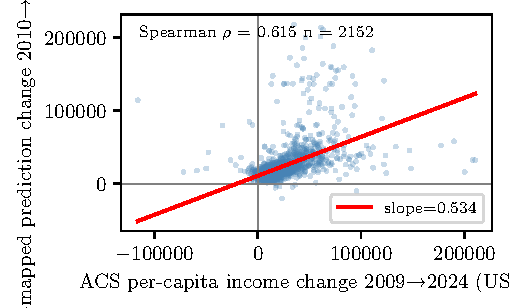
\includegraphics[width=\linewidth]{Figures/C_long_diff_gb2_map.pdf}
    \caption{Long-difference scatter: ACS per-capita income change 2009--2024 (horizontal) versus GB2-mapped model prediction change 2010--2024 (vertical). The positive slope confirms directional consistency, but the modest correlation reflects the model's inability to detect income changes without a corresponding physical footprint.}
    \label{fig:longdiff}
\end{figure}

\textbf{SUPER EARLY DRAFT. NEED IDEAS FOR THIS SECTION.}

\textbf{TODO: Add a specific case-study neighborhood (e.g., Hudson Yards or DUMBO) to provide a qualitative, spatially-anchored illustration. Consider reserving a compact geographic cluster in the test set (rather than purely random tract assignment) so the case study draws on fully held-out buildings. See evaluation.py Part E for the Hudson Yards case-study infrastructure already implemented.}

\section{Conclusions}\label{sec:conclusions}
% Left blank per author instructions.

\bibliographystyle{apa}
\bibliography{references} % Entries are in the refs.bib file



\end{document}

